%\documentclass[12pt,a4paper]{article}
\documentclass[12pt,a4paper]{scrartcl}
%\documentclass[11pt,a4paper,oneside]{book}
% ===================== PACKAGES =====================
\usepackage[british]{babel}
\usepackage[tmargin=1in, bmargin=1in, lmargin=0.75in, rmargin=0.75in]{geometry}
\usepackage[dvipsnames,table]{xcolor}  % prima di tikz, listings, ecc.

\usepackage{tikz}
\usepackage{graphicx}
\usepackage{pgfplots}
\pgfplotsset{width=12cm, compat=1.9}
\usepackage{setspace}
\usepackage{chemmacros}
\usepackage{chemfig}
\usepackage{esint}
\usepackage{tabularray}
\usepackage{makeidx}
\usepackage{epstopdf}
\usepackage{amssymb}
\usepackage{mathrsfs}
\usepackage{bm}
\usepackage{amsmath}
\usepackage{enumitem}
\usepackage[english]{varioref}
\usepackage{lipsum}
\usepackage{fancyhdr}
\usepackage{float}
\usepackage{empheq}
\usepackage[framemethod=tikz]{mdframed}
\numberwithin{equation}{section}
\usepackage{eso-pic}
\usepackage{calc}
\usepackage{nccmath}
\usepackage{caption}
\usepackage{subcaption}
\usepackage{gensymb}
\usepackage{amsfonts, amsthm, epsfig, epstopdf, titling, url, array}
\usepackage{tabularx}
\usepackage{makecell}
\usepackage{booktabs}
\usepackage{array}
\usepackage{siunitx}
\sisetup{input-digits=0123456789\pi}
\usepackage[symbol]{footmisc}
\usepackage{multicol}
\usepackage{boondox-cal}
\usepackage{blindtext}
\usepackage{changepage}
\usepackage{nomencl}
\usepackage{hyperref}
\usepackage{xurl}
\usepackage{ragged2e}
\usepackage[version=4]{mhchem}  % ← conflitto di opzioni
\usepackage{longtable}
\usepackage{chemformula}
\usetikzlibrary{arrows.meta,positioning,calc}

% ===================== SI UNITS =====================
\DeclareSIUnit\atm{atm}
\DeclareSIUnit{\var}{var}
\DeclareSIUnit{\pu}{p.u.}


% ===================== MATH OPERATORS =====================
\DeclareMathOperator{\rank}{rank}
\DeclareMathOperator{\atantwo}{atan2}
\DeclareMathOperator{\spn}{span}

% ===================== COMMANDS =====================
\newcommand{\abs}[1]{\left|#1\right|}
\newcommand{\sign}{\text{sign}}
\newcommand{\centered}[1]{\begin{tabular}{@{}l@{}} #1 \end{tabular}}

% ===================== COLORS =====================
\definecolor{mycolor1}{rgb}{0.97, 0.97, 0.97}
\definecolor{mycolor2}{rgb}{0.97, 0.97, 0.97}
\definecolor{tableShade}{gray}{0.9}

% ===================== THEOREM ENVIRONMENTS =====================
\theoremstyle{it}
\newtheorem{defn}{Definition}[section]
\newtheorem{assumption}{Assumption}[section]
\newtheorem{thm}{Theorem}[section]
\newtheorem{lemma}{Lemma}[section]
\newtheorem{corollary}{Corollary}[section]
\theoremstyle{definition}
\newtheorem{example}{Example}[section]

% ===================== CUSTOM ENVIRONMENTS =====================
\newenvironment{myitemize_1}{
	\begin{itemize}[topsep=0pt]
		\setlength{\topsep}{2pt}
		\setlength{\itemsep}{2pt}
		\setlength{\parskip}{2pt}
		\setlength{\parsep}{2pt}
	}{\end{itemize}}

\newmdenv[
innerlinewidth=0.5pt,
roundcorner=4pt,
backgroundcolor=mycolor2,
linecolor=mycolor1,
innerleftmargin=6pt,
innerrightmargin=6pt,
innertopmargin=6pt,
innerbottommargin=6pt
]{mybox}

% ===================== TABLE COLUMN TYPES =====================
\newcolumntype{Y}{>{\hsize=2\hsize}X}
\newcolumntype{Z}{>{\centering\arraybackslash\hsize=0.857\hsize}X}

% ===================== SECTION DEPTH =====================
\setcounter{secnumdepth}{3}
\setcounter{tocdepth}{3}

% ===================== PAGE STYLE =====================
\setlength{\headheight}{20pt}
\setlength{\headsep}{20pt}

\pagestyle{fancy}
\fancypagestyle{firstpage}{\rhead{}}
\fancyhead[L]{\slshape\nouppercase{\leftmark}}
\chead{}
\rhead{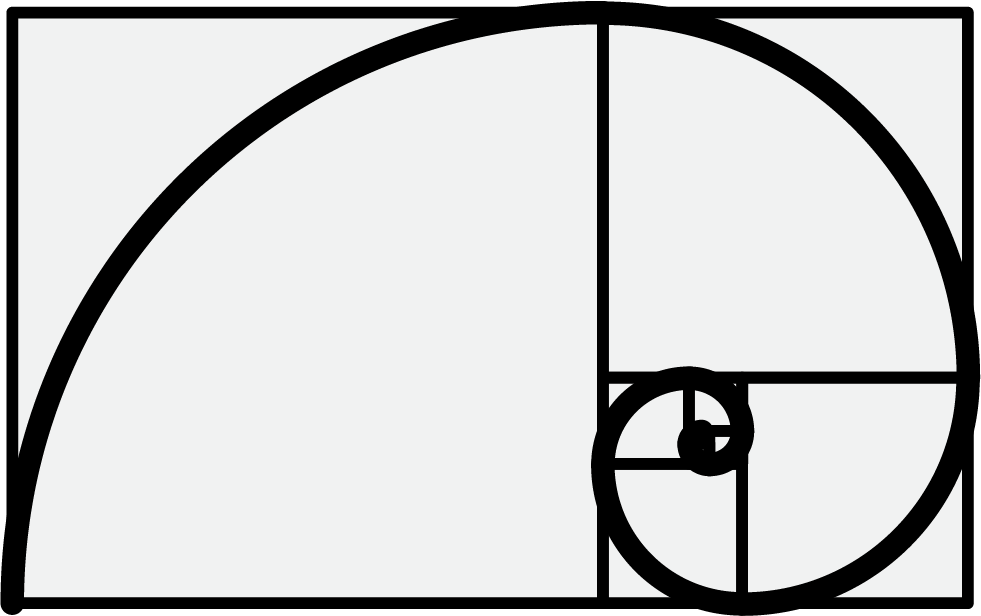
\includegraphics[height=0.75cm]{../../AAA_template_latex_settings/pwr-control_logo_doc.png}}
\lfoot{\href{http://www.pwr-control.com}{pwr-control.com}}
\cfoot{-\ \thepage\ -}
\rfoot{\textit{}}
\renewcommand{\headrulewidth}{0.4pt}
\renewcommand{\footrulewidth}{0.4pt}


\geometry{
	a4paper,
	top    = 2.5cm,
	bottom = 3.0cm,
	left   = 2.5cm,
	right  = 2.5cm
}

\hypersetup{
	colorlinks = true,
	urlcolor   = blue,
	linkcolor  = black,
	citecolor  = black
}

\pagenumbering{gobble}

% =============================================================
%  
% =============================================================

\newcommand{\DocCategory}{Technical Research Report}
\newcommand{\DocField}{Power Electronics and Control Systems}

\newcommand{\DocTitle}{%
	{\fontsize{20}{24}\selectfont\bfseries Long Power Cable Effects:} \\[16pt]
	{\fontsize{16}{20}\selectfont\bfseries in electrical drives.}
}

\newcommand{\DocSubtitle}{%
	Investigation of shielded power cable and its impact on electrical drive performances. 
}

\newcommand{\DocAuthor}{Davide Bagnara}
\newcommand{\DocDate}{July 2026}

\newcommand{\DocAbstract}{%
	This report investigates the acoustic emission radiated by the long shielded three-phase cable connecting the inverter to the machine. A specific installation is examined in which the cable run produces audible noise under PWM operation: the emission shows a tonal component at the converter switching frequency, spreads into broadband noise when random PWM is applied, and is present on the 120 m section while absent on the 40 m one.
	A consistent model is developed that links the differential (positive-sequence) PWM ripple current to the inter-conductor electromagnetic (Ampère) forces, the resulting transverse vibration of the cable spans, and the radiated sound. The analysis indicates that the audible excitation arises from the product of the fundamental current and the switching-frequency ripple, so it is governed by the differential mode rather than the common mode, and that the length dependence follows from a resonant coupling between the force harmonics and the mechanical modes of the cable spans. Experimental and simulation results are included to support the proposed explanation.
}


% Tre righe metadati in fondo (label small caps + valore)
\newcommand{\MetaLabelA}{Project Repository}
\newcommand{\MetaValueA}{https://github.com/pwr-control/modelization-and-control.git}
\newcommand{\MetaValueAUrl}{https://github.com/pwr-control/modelization-and-control.git}
\newcommand{\MetaValueALabel}{modelization-and-control.git}


\newcommand{\MetaLabelB}{Framework}
\newcommand{\MetaValueB}{MATLAB/Simulink/Simscape}

\newcommand{\MetaLabelC}{Architecture}
\newcommand{\MetaValueC}{SiC, EiceDRIVER, Customized Power Supplies}

% =============================================================
%  FRONTESPIZIO
% =============================================================
\begin{document}
	\titlepage
	% ---- Intestazione centrata ----
	\begin{center}
		{\Large\scshape \DocCategory}\\[8pt]
		{\large\scshape \DocField}
	\end{center}
	
	\vspace{36pt}
	\noindent\rule{\linewidth}{0.8pt}
	
	% ---- Titolo ----
	\vspace{16pt}
	\begin{center}
		\DocTitle
	\end{center}
	
	\vspace{4pt}
	\noindent\rule{\linewidth}{2.2pt}
	
	% ---- Sottotitolo ----
	%\vspace{14pt}
	\begin{center}
		\begin{onehalfspace}
			{\large\itshape \DocSubtitle}
		\end{onehalfspace}
	\end{center}
	
	% ---- Spazio prima di Autore/Data ----
	\vspace{18pt}
	
	% ---- Author / Date su due colonne ----
	\begin{minipage}{0.92\linewidth}
		\noindent
		\begin{minipage}[t]{0.48\linewidth}
			\textbf{Author:}\\[2pt]
			\DocAuthor
		\end{minipage}%
		\hfill
		\begin{minipage}[t]{0.48\linewidth}
			\raggedleft
			\textbf{Date:}\\[2pt]
			\DocDate
		\end{minipage}
	\end{minipage}
	% ---- Spazio prima dell'abstract ----
	\vspace{36pt}
	
	% ---- Abstract indentato ----
	\begin{center}
		\begin{minipage}{0.85\linewidth}
			%    \small
			\footnotesize 
			\begin{onehalfspace}
				\textbf{Abstract:} \DocAbstract
			\end{onehalfspace}
		\end{minipage}
	\end{center}
	
	% ---- Spazio prima dei metadati ----
	\vfill
	
	% ---- Metadati in fondo ----
	\noindent
	\begin{tabular}{@{} r @{\quad} l @{}}
%		\textsc{\MetaLabelA:} & {\url{\MetaValueA}} \\[3pt]
		\textsc{\MetaLabelA:} & {\href{\MetaValueAUrl}{\MetaValueALabel}} \\[3pt]
		\textsc{\MetaLabelB:} & {\MetaValueB}       \\[3pt]
		%		\textsc{\small\MetaLabelC:} & {\small\MetaValueC}       \\
	\end{tabular}
	
	% =============================================================
	%  Fine frontespizio
	% =============================================================
	\newpage
	\pagenumbering{arabic}
	\setcounter{page}{1}
	\tableofcontents
	\listoffigures	
	\listoftables
	\newpage
	
\begin{onehalfspace}	
\section{Introduction}	
To introduce the work described along the document, it could be useful to start from a generic configuration which the \textit{ElectricalDrive} are subjected, as shown in Figure~\ref{ElectricalDrive_connection_figure_1b}.
\begin{figure}[H]
	\centering
	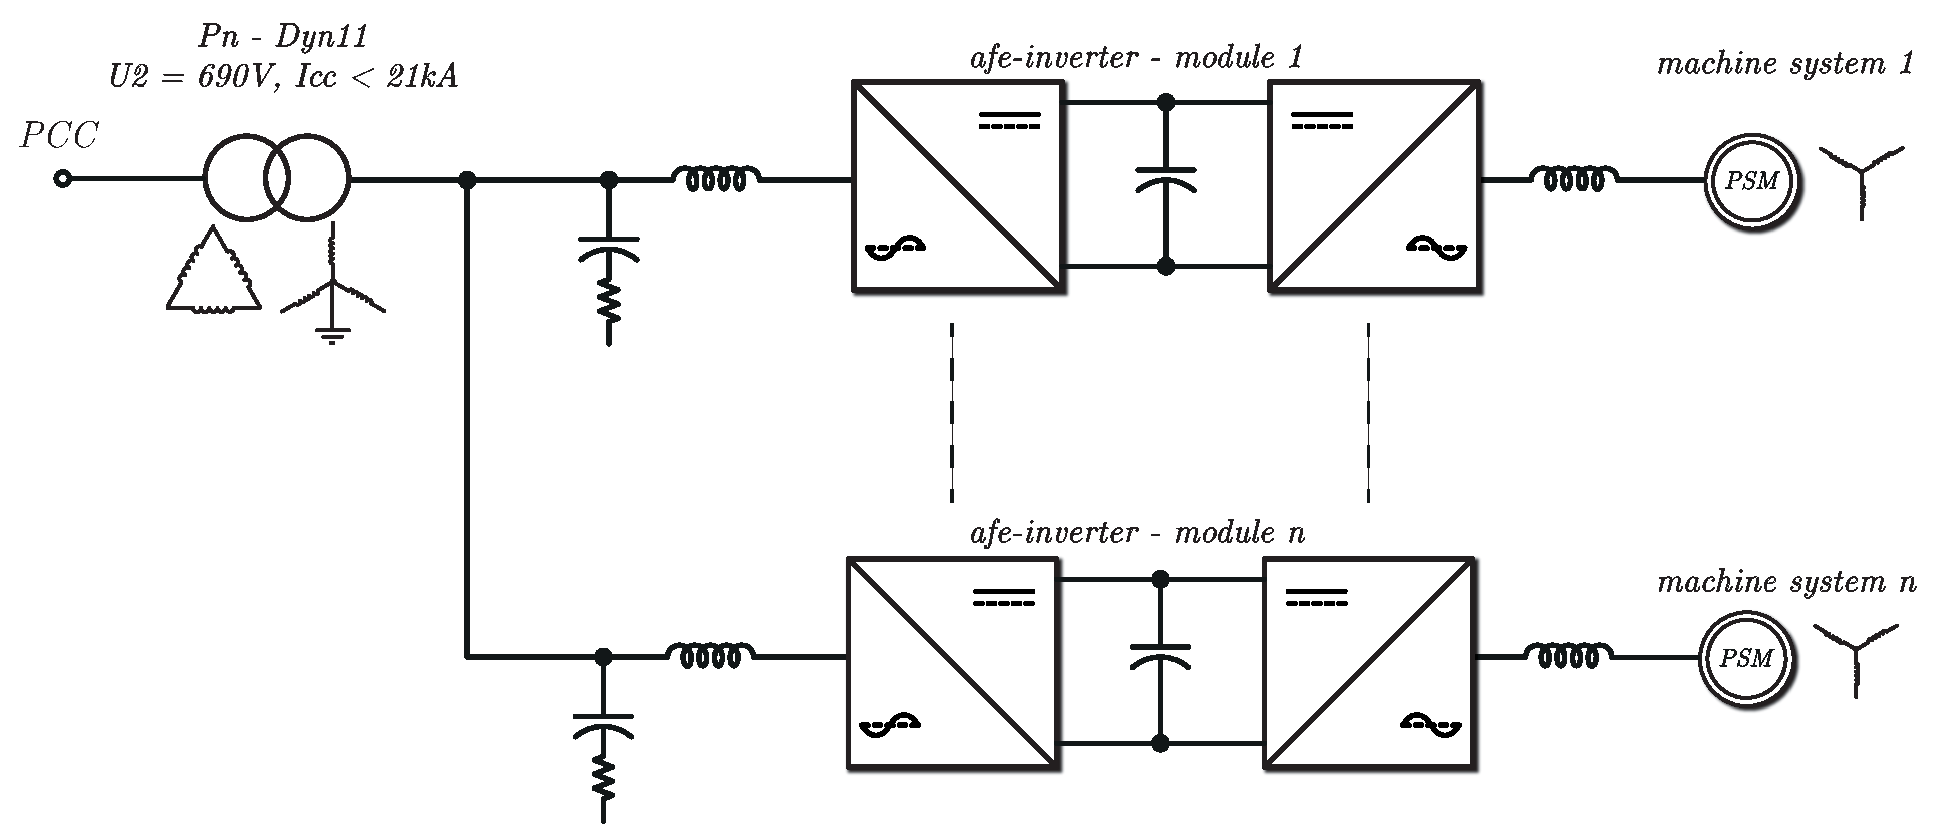
\includegraphics[width = 450pt, angle = 0, 
	keepaspectratio]{figures/ElectricalDrive_connection.eps}
	\captionsetup{width=0.75\textwidth, font=small}	
	\caption{Functional representation of the electrical drives (\textit{ElectricalDrive}) configuration respect to the PSM modularity and the grid connection. Each, galvanically isolated three phase system of the PSM has been connected to a specific electrical drive.}
	\label{ElectricalDrive_connection}
\end{figure}



\begin{thebibliography}{99}
	\bibitem{ieee_519} 
	IEEE SA, \emph{IEEE Standard for Harmonic Control in Electric Power Systems}. IEEE Power and Energy Society. IEEE Std 519 2022 (Revision of IEEE 519-2014).
\end{thebibliography}

%*********************************************************
% Print bibliography (If bibliography is empty nothing happens)
%*********************************************************
%\newpage
%\printbibliography[heading=bibintoc]
\end{onehalfspace}
\end{document}